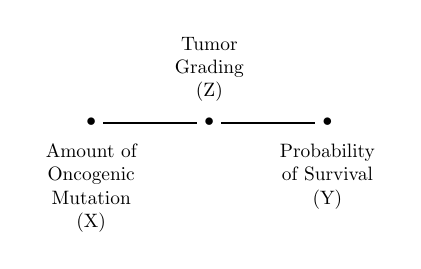
\begin{tikzpicture}[thick, scale=0.5, every node/.style={scale=0.7}]{
            \node [label=below: \begin{tabular}{c} Amount of \\ Oncogenic \\ Mutation \\ (X)\end{tabular}] (a) at (7,3) {$\bullet$};
            \node [label=above:\begin{tabular}{c} Tumor \\ Grading \\ (Z)\end{tabular}] (s) at (10,3) {$\bullet$};
            \node [label=below: \begin{tabular}{c} Probability  \\ of Survival  \\ (Y)\end{tabular}] (x) at (13,3) {$\bullet$};
            \path (a) edge (s);
            \path (s) edge (x);
        } 
        \end{tikzpicture}